\documentclass[11pt]{article}
\usepackage{../cs170}

\def\title{Homework 2}
\def\duedate{Monday 9/11/2023, at 10:00 pm (grace period until 11:59pm)}
\urlstyle{same}

\begin{document}
\maketitle
Due \textbf{\duedate}

\question{Study Group}
List the names and SIDs of the members in your study group.
If you have no collaborators, you must explicitly write ``none''.

\begin{solution}
	None.
\end{solution}

\question{Two sorted arrays}

You are given two sorted arrays of integers, each of size $k$. 
Give an efficient (i.e., better than $O(k)$-time) algorithm to find the $k$-th smallest element in the union of the two arrays. You may assume that all the elements are distinct. 

Your solution should contain a description of the algorithm, a proof of correctness and runtime analysis. (i.e a \href{https://cs170.org/resources/homework-guidelines/}{ 3-part solution}). \textbf{In addition, please provide corresponding pseudo-code.}

\begin{solution}
	My algorithm is as follows: Call the arrays $A$ and $B$. Take the $\frac{k}{2}$-th element of both arrays, 
	and compare the two. The larger of the two will be the $k$-th smallest element. 

	Now for the proof of correctness: since both arrays are sorted, then the union of the first 
	$\frac{k}{2}$ elements of both arrays will form the $k$ smallest elements of the array. This is because 
	the arrays are sorted so any element larger than the $\frac{k}{2}$-th element will be larger than 
	$\frac{k}{2}$ elements, and hence it cannot appear in the first $k$-elements. Picking the larger of the two
	ensures that we pick the $k$-th smallest element, since it's the largest element in the first $k$ elements.

	As for the runtime analysis, accessing array elements are constant time, and comparing them is also 
	constant time. Therefore, this algorithm actually executes in $\Theta(1)$ time. Here's the pseudocode 
	for the program, I couldn't get the latex to work so I just pasted pseudocode I wrote in VSCode 
	(in the meantime I'll try to get the Latex working):

	\begin{center}
		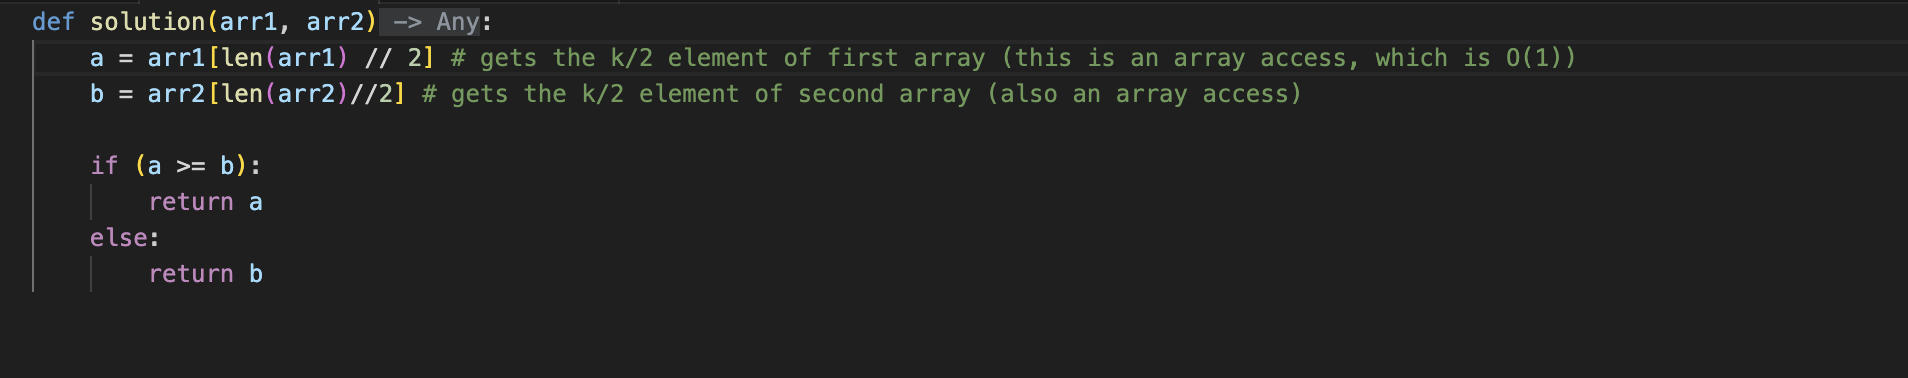
\includegraphics[scale=0.5]{code.png}
	\end{center}
\end{solution}
\pagebreak
\question{Counting multiples of 3}

You are given an array $A$ of $n$ distinct non-negative integers. Give an $O(n (\log n)^2)$ time algorithm to count the number {\bf odd}-sized subsets of $A$ whose elements add up to a multiple of $3$. 

You can assume that multiplying two $k$ bit integers can be done in $O(k \log k)$ time (see \href{https://annals.math.princeton.edu/2021/193-2/p04}{Harvey and van der Hoeven}). 

\emph{Hint 1: Note that the number of such subsets can scale exponentially with $n$, so we cannot assume that arithmetic operations take $O(1)$ time. To bound the cost of adding and multiplying, show that the number of subsets of a size $n$ array can be stored in an $n$-bit integer.} 

\emph{Hint 2: Try keeping track of the number of odd and even sized subsets that sum to 0, 1, or 2 mod $3$ using divide and conquer. How do you combine the subproblems of size $k$ in $O(k \log k)$ time?}

\begin{solution}
	First, we follow the first hint and show that the number of subsets can be stored in an $n$-bit integer. 
	We know that for $n$ bits, the largest number we can store is $2^n$ (assuming unsigned integers here). 
	However, the total number of subsets (i.e. the total number of partitions) is given by the equation:
	\[
		N = {n \choose 1} + {n \choose 2} + \dots + {n \choose n} = \sum_{i = 1}^N {n \choose i} = 2^n
	\] 
	Therefore, we can store exactly the total number of subsets in an $n$-bit integer. This will be important 
	later, when we will be storing number of subsets with conditions later on, and multiplying them together. 

	Now consider a set $A$. First, we can take modulo 3 for all the elements, giving us an array consisting
	only of 0, 1, 2. This step can be done prior to running the recursive algorithm, and takes $O(n)$ time, which
	we will show later on to not really matter. 
	 
	Now, let's split the array $A$ into two parts, $A_L$ and $A_R$ for the left and right portions. At each 
	layer, we will recursively divide our array into a left and right portion, and run our function on those
	smaller subproblems. For an array of size $n$, this takes $\log n$ steps to get down to a subproblem of size
	1. 

	Now suppose we have the two arrays $A_L$ and $A_R$. There are six values we are interested, as alluded to by
	hint 2: the number of odd and even sizes subsets that sum to 0, 1, or 2 modulo 3; specifically, call these 
	values $E_0$, $E_1$, $E_2$, $O_0$, $O_1$, $O_2$, where the letter denotes whether the subsets are even or 
	odd in size, and the subscript denotes what it sums to modulo 3. We will then add another subscript $L$ 
	and $R$ to show whether the number is from $A_L$ or $A_R$. Now, we do the following to combine: 
	\begin{itemize}
		\item To generate $O_0$, we compute $O_{0L}E_{0R} + E_{0L}O_{0R} + O_{1L}E_{2R} + E_{1L}O_{2R} +
			O_{2L}E_{1R} + E_{2L}O_{1R}$.
		\item To generate $E_0$, we compute $O_{0L}O_{0R} + E_{0L}E_{0R} + O_{1L}O_{2R} + E_{1L}E_{2R} + 
			O_{2L}O_{1R} + E_{2L}E_{1R}$. 
		\item To generate $O_1$, we compute $O_{0L}E_{1R} + E_{0L}O_{1R} + O_{1L}E_{0R} + E_{1L}O_{0R} + 
			O_{2L}E_{2R} + E_{2L}O_{2R}$.
		\item To generate $E_1$, we compute $O_{0L}O_{1R} + E_{0L}E_{1R} + O_{1L}O_{0R} + E_{1L}E_{0R} +
			O_{2L}O_{2R} + E_{2L}E_{2R}$.
		\item To generate $O_2$, we compute $O_{0L}E_{2R} + E_{0L}O_{2R} + O_{1L}E_{1R} + E_{1L}O_{1R} +
			O_{2L}E_{0R} + E_{2L}O_{0R}$.
		\item To generate $E_2$, we compute $O_{0L}O_{2R} + E_{0L}E_{2R} + O_{1L}O_{1R} + E_{1L}E_{1R} +
			O_{2L}O_{0R} + E_{2L}E_{0R}$.	
	\end{itemize}
	To show that this combination step happens in $O(k \log k)$ time, we know that each one of these numbers 
	is less than $2^k$ since they count a subset of the number of subsets. Since this is the case, they 
	can be stored in a $k$-bit integer. Then, the multiplication of two $k$-bit integers is $O(k \log k)$, 
	so therefore the combination indeed does take $O(k \log k)$ time. 

	Therefore, we have the current situation: Each subproblem takes $O(k \log k)$ time (which is the same as 
	$O(n \log n)$ time since the problem size at each level is dependent on $n$), and we have $\log n$ problems.
	Therefore, we have to take the product of the two to get our final runtime, which is:
	\[
		\log n \cdot O(n \log n) = O(n (\log n)^2)
	\] 
\end{solution}
\pagebreak
\question{The Resistance}

We are playing a variant of The Resistance, a board game where there are $n$ players, $s$ of which are spies. In this variant, in every round, we choose a subset of players to go on a mission. A mission succeeds if the subset of the players does not contain a spy, but fails if at least one spy goes on the mission. After a mission completes, we only know its outcome and not which of the players on the mission were spies.

Come up with a strategy that identifies all the spies in $O(s \log (n/s))$ missions. \textbf{Describe your strategy and analyze the number of missions needed.}

\begin{solution}
	We split the initial group into $\frac{n}{s}$ groups, and have all of them go on a mission. Of the ones 
	that succeed, we can safely eliminate those people as being spies, and we can focus our attention on the 
	missions that do fail. 

	Of the missions that do fail, we can now use binary search to help us find where the spies are. 
	Here, we would recursively split into two groups and send them on a mission, then of those groups
	that fail we can split into two's again. Since this algorithm emulates binary search then they share the same
	runtime, which is $O(\log(k))$ where $k$ is the size of the initial array. Since our arrays are of 
	size $\frac{n}{s}$, then this operation takes $O(\log(n / s))$ time. This means that for 
	each subproblem of size $\frac{n}{s}$, we have $O(\log (n / s))$ runtime. 

	Now let's look at how many times we need to run this algorithm. In the worst case scenario, we happen to 
	divide the $s$ groups in such a way that there is exactly one spy per group. This means that all the 
	initial missions will fail, and we will have to perform binary search on every single subgroup. This 
	is the worst case, where we have to run an our algorithm $s \cdot \log(n / s)$ times, so our total 
	runtime (since it's an upper bound), will be $O(s \log (n / s))$. 
\end{solution}
\pagebreak
\question{Werewolves}
You are playing a party game with $n$ other friends, who play either as werewolves or humans.
You do not know who is a human and who is a werewolf, but all your friends do.
There are always more humans than there are werewolves.

Your goal is to identify one player who is certain to be a human.

Your allowed `query' operation is as follows: you pick two players as partners. You ask each player if their partner is a human or a werewolf.
When you do this, a human must tell the truth about the identity of their partner,
but a werewolf doesn't have to (they may lie or tell the truth about their partner).

Your algorithm should work regardless of the behavior of the werewolves.

\begin{subparts}
	\subpart For a given player $x$, devise an algorithm that returns whether or not $x$ is a human using $O(n)$ queries. Just an informal description of your test and a brief explanation of why it works is needed.

	\begin{solution}
		We pair $x$ with $n$ different people. Then, on each pair, we ask $x$ and their partner to identify 
		each other. 
		If $x$ identifies everybody as a human, or identifies more werewolves than humans, then they are 
		immediately a werewolf, since this cannot be true. Therefore, this means that $x$ must identify 
		at least one werewolf, but still preserve the fact that there are more humans than werewolves.

		Now, consider everybody that $x$ has identified as a human. Note that because humans form the majority 
		in the group, then this implies that \textit{at least} one human is present in the list of people that
		$x$ identifies as human. To really show the power of this conclusion, we need to look at what these 
		``humans'' identified $x$ as. 

		Note that since this group of people are all ``humans,'' then their identification of $x$ must all 
		be consistent (i.e. they must all identify $x$ as either human or werewolf) otherwise $x$ must be a werewolf.
		This is because we know that humans can only tell the truth, so if one ``human''
		identifies $x$ as human but another identifies $x$ as a werewolf, then we know that one of the two 
		must have been lying, hence they cannot be both human, so $x$ was lying, meaning that $x$ was a werewolf.
		
		Combining this with the earlier conclusion that at least one true human exists within this group, 
		it means that all the werewolves have to align their identifications with the identification that 
		human gives, which we know must be truthful. Therefore, if they all identify $x$ as human,
		then $x$ is certainly human, and if they 
		all identify $x$ as a werewolf, then $x$ is certainly a werewolf. 
	\end{solution}
	
	\subpart Show how to find a human in $O(n\log n)$ queries (where one query is taking two players $x$ and $y$ and asking $x$ to identify $y$ and $y$ to identify $x$).
	
	\textit{Hint: Split the group into two groups, and use part (a). What invariant must hold for at least one of the two groups?}

	\textbf{Give a \href{https://cs170.org/resources/homework-guidelines/}{3-part solution}.}

	\begin{solution}
		I've combined the description and the proof of correctness into one (sorry in advance, I realized 
		that I had to split these up too late): 

		On each problem, we split into two groups (as alluded to by the hint), and we know that in at least 
		one of the two groups it is the case that there are more humans than werewolves. Further, 
		since this is invariant across all layers of the tree, then this means that there is a ``trail'' 
		of human-majority subgroups all the way down. This means that at the bottom of the tree, we are 
		guaranteed to have at least one true human. We now have to figure out how to combine subproblems.

		Consider the ``trail'' where there is a human majority. At the bottom of the tree, we know that 
		the player returned by this branch is guaranteed to be a human, whereas we can't say anything about 
		the other branches. To combine the subproblems, consider the two players that are ``nominated'' by 
		the algorithm; one of these is a true human, the other is a false human. To determine the truthfulness
		of these players, we can run the algorithm from part (a)
		on these two people with the combined group of players, which will determine which of the two 
		came from the human-majority subgroup (this player we will be able to confirm is human from part (a)), 
		and which one came from the werewolf-majority subgroup. If they both 
		succeed, then we can nominate either of them to the layer above, since they're both confirmed to be human. 
		from part (a).

		Since all the nominees must ``encounter'' the true human at some point in the recursion tree (as in 
		they will all be compared to the true human at some point) and the true human cannot fail the test
		in part (a), then we guarantee that we can identify at least one true human at the end of the algorithm.


		A quick analysis on the runtime: At each layer, the time it takes to combine the subgroups 
		together takes $O(2n) = O(n)$ time, and since we are halving at each layer, then there are $\log n$ 
		layers to perform this calculation, so taking the product of these two gets us the 
		total runtime: $O(n \log n)$, as desired.
	\end{solution}

	\subpart (\textbf{Optional, not for credit}) Can you give a $O(n)$ query algorithm?
	
	\textit{Hint: Don't be afraid to sometimes `throw away' a pair of players once you've asked them to identify their partners.}

	\textbf{Give a \href{https://cs170.org/resources/homework-guidelines/}{3-part solution}.}

\end{subparts}

\newpage

\question{[Coding] Quickselect}

For this week's homework, you'll implement the quickselect algorithm in a python jupyter notebook called \texttt{quickselect.ipynb}. There are two ways that you can access the notebook and complete the problems:
\begin{enumerate}
    \item \textbf{On Local Machine}: \texttt{git clone} (or if you already have it, \texttt{git pull}) from the coding homework repo, 
    
    \href{https://github.com/Berkeley-CS170/cs170-fa23-coding}{\texttt{https://github.com/Berkeley-CS170/cs170-fa23-coding}}
    
    and navigate to the \texttt{hw02} folder. Refer to the \texttt{README.md} for local setup instructions.

    \item \textbf{On Datahub}: Click \href{https://datahub.berkeley.edu/hub/user-redirect/git-pull?repo=https%3A%2F%2Fgithub.com%2FBerkeley-CS170%2Fcs170-fa23-coding&urlpath=tree%2Fcs170-fa23-coding%2Fhw02%2Fquickselect.ipynb&branch=main}{here} and navigate to the \texttt{hw02} folder if you prefer to complete this question on
Berkeley DataHub.
\end{enumerate}

\noindent Notes:
\begin{itemize}
    \item \textit{Submission Instructions:} Please download your completed \texttt{quickselect.ipynb} file and submit it to the gradescope assignment titled ``Homework 2 Coding Portion''. 
    
    \item \textit{OH/HWP Instructions:} Designated coding course staff will provide conceptual and debugging help during office hours and homework parties.
    
    \item \textit{Academic Honesty Guideline:} We realize that code for some of the algorithms we ask you to implement may be readily available online, but we strongly encourage you to not directly copy code from these sources. Instead, try to refer to the resources mentioned in the notebook and come up with code yourself. That being said, we \textbf{do acknowledge} that there may not be many different ways to code up particular algorithms and that your solution may be similar to other solutions available online.
    
\end{itemize}

\end{document}

